\chapter{Konzeption der Softwarelösung}
\label{chap:konzeption_der_softwareloesung}

\section{Machine Learning Modell} %TODO: eigenes chapter hierfür! (Analyse der verschiedenen NLP Modelle in Bezug auf Fake News Erkennung)

\subsection{Welches Modell für Fake News Erkennung?}
%TODO: ML, DL oder Hybrid (Bow, TD-idf oder word embeddings)
\cite{sharma2025}

\begin{figure}[htbp]
    \begin{center}
        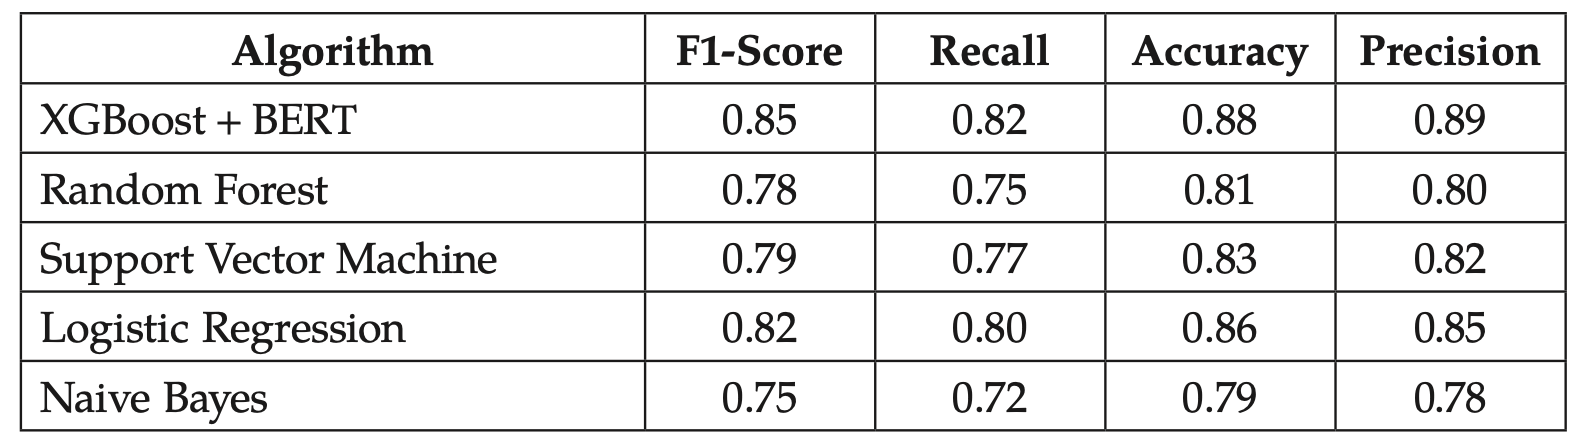
\includegraphics[scale=0.5]{static/xgboost_bert.png}
        \caption{\label{fig:xgboost_bert} Vergleich ... \cite{sharma2025}}
    \end{center}
\end{figure}

Word2vec + LSTM \cite{matheven2022}

\subsubsection{XGBoost}

%TODO: Informationen prüfen


In der Studie von \cite{petrovic2024} wurde XGBoost mit der TF-IDF-Vektorisierung kombiniert, 
um Fake News aus textuellen Inhalten zu identifizieren. Durch eine zusätzliche Hyperparameter-Optimierung mittels eines 
metaheuristischen Verfahrens (VNS) konnte die Modellleistung weiter verbessert werden. Die Autoren betonen, 
dass XGBoost durch die Integration von Regularisierung und adaptiver Lernstrategie eine exzellente Eignung für textklassifikatorische 
Aufgaben zeigt.

In einer weiteren aktuellen Studie wurde XGBoost in Kombination mit BERT eingesetzt, um Sarkasmus in Texten zu erkennen. 
Diese hybride Architektur kombinierte semantische Einbettungen mit der Klassifikationsstärke von XGBoost und lieferte deutlich bessere 
Ergebnisse als Deep-Learning-Modelle allein \cite{sharma2025}.

Auch in der Emotionserkennung aus Textdaten wurde XGBoost erfolgreich eingesetzt. 
In einer experimentellen Vergleichsstudie erzielte XGBoost einen durchschnittlichen F1-Score von 97{,}86\%, 
was ihn zum leistungsfähigsten klassischen ML-Modell gegenüber SVM und Random Forest machte\cite{paksoy2024}. 
Die Studie nutzte unigram-basierte TF-IDF-Features und zeigte, dass XGBoost bei ausgeglichener Klassenzuordnung besonders effektiv ist.


\section{Hauptkomponente} \label{sec:06:hauptkomponente}

Die Hauptkomponente hat die Aufgabe die Artikel auf den verschiedenen Nachrichtenportalen zu lesen und zu ergänzen.
Hierfür muss erkannt werden auf welcher Seite sich der Nutzer befindet. Außerdem muss das html dieser Seite ausgelesen und analysiert werden können.

\paragraph{Als Beispiel die Seite Bild.de:} 
Je nach Fenstergröße hat die Seite entweder die Domäne \textit{https://www.bild.de/} oder \textit{https://m.bild.de/}.

Die Startseite ist wie folgt aufgebaut:

\begin{lstlisting} [language=html]
    <!DOCTYPE html>
    <html>
      <head>
        ...
      </head>
      <body>
        <div id="app">
            ...
            <div id="page-content">
                <header/>
                    <main>
                    <!-- Es gibt auf der Startseite 
                    ueber 50 dieser section-Elemente -->
                        <section>
                            <article/>
                        </section>
                    </main>
                <footer/>
            </div>    
        </div>
      </body>
    </html>
\end{lstlisting}

Wenn ein Artikel geöffnet ist, ist der DOM dem der Startseite sehr ähnlich. Der einzige wesentliche Unterschied ist, dass im \textit{main}-Element
nur noch ein \textit{article}-Element ist und nicht beliebig viele \textit{section}-Elemente.
Ob ein Artikel geöffnet ist, kann also anhand der Anzahl der \textit{article}-Elemente bestimmt werden.

\begin{lstlisting} [language=html]
    <article>
        <h2 class="document-title document-title-article">
            <span class="kicker">Kicker des Artikels</span>
            <span class="headline">Titel des Artikels</span>
        </h2>
    </article>
    <div class="article-body">
        <!-- Pro Artikel gibt es ca. 10 p-Elemente -->
        <p>Inhalt des Artikels</p>
    </div>
\end{lstlisting}

Der Titel und Inhalt des Artikels kann den entsprechenden html-Elementen entnommen werden.
Diese werden dann an die API gesendet und dort verarbeitet. 
Der Rückgabewert der API enthält dann die Info ob der Artikel falsch oder echt ist.
Diese wird in einem von der Hauptkomponente erzeugten \textit{div}-Container über dem Artikel eingefügt.

\begin{table}[ht]
    \centering
    \renewcommand{\arraystretch}{1.3}
    \begin{tabular}{|p{2.5cm}|p{2.5cm}|p{2.5cm}|p{2.5cm}|p{2.5cm}|}
        \hline
        \textbf{Kriterium} & \textbf{Chrome Extension} & \textbf{Userscript (Tampermonkey)} & \textbf{Proxy-Server} & \textbf{Scraper + Plattform} \\
        \hline
        DOM-Zugriff beim Nutzer & Ja & Ja & Nein & Nein \\
        \hline
        Einbindung auf \texttt{bild.de} direkt & Ja & Ja & Ja (indirekt) & Nein \\
        \hline
        Installation durch Nutzer & Mittel & Einfach & Nicht erforderlich & Nicht erforderlich\\
        \hline
        Komplexität der Umsetzung & Mittel & Gering & Hoch & Mittel \\
        \hline
        Wartbarkeit \& Updates & Gut & Gut & Aufwändig & Mittel \\
        \hline
        Performance beim Nutzer & Hoch & Hoch & Hoch & Hoch \\
        \hline
        Skalierbarkeit & Hoch & Eingeschränkt & Mittel & Hoch \\
        \hline
        Für öffentliche Verbreitung geeignet & Ja & Eingeschränkt & Eingeschränkt & Ja \\
        \hline
        API-Nutzung zur Fake-Erkennung & Ja & Ja & Ja & Ja \\
        \hline
        Entwickler-kontrolle über UI & Hoch & Mittel & Hoch & Mittel \\
        \hline
    \end{tabular}
    \caption{Vergleich verschiedener technischer Umsetzungsansätze}
    \label{table:technischeAnsaetze}
\end{table}

Zur Bestimmung des geeignetsten Tools um diese Anforderungen umzusetzen wurden verschiedene Umsetzungsansätze verglichen (siehe \ref{table:technischeAnsaetze}).
Aufgrund des begrenzten Zugriffs auf die zu analysierende Seiten, bieten sich die beiden Client-seitigen Umsetzungen 
eine Chrome Extension zu implementieren oder über Tampermonkey Userscripts auszuführen am ehesten an.

Im Vergleich zu Usercripts unterstützt die Extension mehrere Komponenten (Content Scripts, Background Scripts, Popup, Optionsseite).
Anhand dieser können der DOM beobachtet, ein persistenter Speicher genutzt, Kontextmenüs erstellt und auf Browseraktionen reagiert werden (z.B. Tabwechsel, Navigation).
Ein Userscript hingegen ist ein einfaches Script, das nur beim Laden einer Seite aktiv ist und dementsprechend keine Hintergrundverarbeitung und keine erweiterten UI-Komponenten
zur Verfügung stellt.

Zur Implementierung der Hauptkomponente wird also eine Chrome Extension genutzt.

    
    
    